\section{Design und Implementierung}
\subsection{Auswahl des Reglers}
\autor{Aaron J. Müller}
Im direkten Vergleich liefert \gls{MPC} ein deutlich besseres Regelverhalten als der Stanley Regler \cite{stanley_mpc_comparison1}\cite{stanley_mpc_comparison2}. 
Durch die Entscheidung, bei Hardwareupgrades eine hohe Rechenleistung zu präferenzieren, ist die aufwändigere Berechnung der Simulation und Optimierungsfunktion auch realisierbar.
Als weiteren Vorteil ist, dass eine \gls{MPC}-Regler auch als \gls{MIMO} System entworfen werden kann, um zusätzlich die Aufgabe der Longitudinalregelung zu übernehmen.
Dadurch könnte der bestehende Longitudinalregler im gleichen Schritt durch eine bessere Alternative ersetzt werden.

Entgegen dieser Vorteile wurde jedoch die Entscheidung getroffen, den Stanley-Regler umzusetzen. 
Der treibende Grund hierfür ist der vergleichsweise niedrige Entwicklungsaufwand, sowohl wegen der einfacheren Logik als auch wegen schon bereits bestehender Vorarbeit an einem Stanley-Regler für den it:movES Softwarestack \cite{Nico_Stanley}.
Die Implementierung des \gls{MPC} würde im Gegenzug den Fortschritt des Gesamtprojektes sabotieren, der aufgrund der Teilnahme an der \gls{BFMC} in einem festen Zeitplan gebunden ist.

\subsection{Solltrajektorie}
\autor{Aaron J. Müller}
Eine robuste Solltrajektorie ist essentiell für ein gutes Regelverhalten.
Auch wenn die Generierung der Solltrajektorie nicht direkt Teil der Entwicklung des Reglers ist, so muss doch ein geeignetes Interface definiert werden.
Die bisher verwendete Solltrajektorie stellt die Mitte der aktuell befahrenen Spur dar, und wird durch einen Offset von der Fahrbahnbegrenzung ermittelt.
Der bisherige Regler verwendet dann den \gls{CTE} und die Krümmung, um den Lenkwinkel zu berechnen.

Da der Stanley-Regler stattdessen koordinatenbasiert arbeitet, gibt es zwei mögliche Vorgehensweisen:
\begin{itemize}
    \item Der Regler erhält weiterhin eine parametrische Beschreibung der Trajektorie, und errechnet die benötigten Koordinaten selber
    \item Der Regler erhält die Solltrajektorie direkt als Reihe von Koordinatenpaaren
\end{itemize}

Bei einer kontinuierlichen Kurve kann die Referenzposition genauer gewählt werden.
Im Gegenzug ist die Verarbeitung von Koordinaten einfacher, was vor allem für die Transformation zwischen verschiedenen Koordinatensystemen von Bedeutung ist.

Ein weiterer wichtiger Punkt der berücksichtigt werden sollte, ist dass die Verwendung von Koordinatenpaaren eine flexiblere Berechnung des Sollgierwinkels ermöglicht, näheres dazu wird im späteren Abschnitt \ref{controller-gierwinkel} erläutert.
\newline
Aus den genannten Gründen wurde eine koordinatenbasierte Solltrajektorie gewählt, und als Schnittstelle definiert.
Es gilt noch zu untersuchen, ob die Berechnung der Solltrajektorie wie sie bisher implementiert ist auf Koordinatenpaare angepasst werden kann, oder ob diese durch Abtastung der parametrischen Kurve bestimmt werden müssen.
In beiden Fällen muss Rücksicht auf die Kameraperspektive genommen werden, sodass die errechneten Koordinatenpaare immer einen konstanten Abstand zueinander aufweisen.


\subsection{Sollgierwinkel}
\label{controller-gierwinkel}
\autor{Aaron J. Müller}
Für die Berechnung des Sollgierwinkels aus der Solltrajektorie gibt es grundsätzlich zwei anwendbare Formeln \cite{Nico_Stanley}, welche mit den beiden Darstellungen der Solltrajektorie korrelieren.

Allgemein lässt sich der Sollgierwinkel aus der Fahrgeschwindigkeit $v$ und der Krümmung der Solltrajektorie, $\kappa_{ref,W}$, berechnen (Formel \ref{sollgierwinkel_krümmung}).
Dabei ist zu beachten, dass die Krümmung an der gewählten Referenzposition verwendet wird. 
Es ist also ungünstig, die Krümmung der gesamten Trajektorie, so wie sie in der Parabeldarstellung der Solltrajektorie enthalten ist, zu verwenden.

\begin{equation}
\label{sollgierwinkel_krümmung}
\psi_{ref,W}=v\kappa_{ref,W}=\frac{v}{r_{ref,W}}
\end{equation}

Durch umformen lässt sich Formel \ref{sollgierwinkel_geschwindigkeiten} bilden, welche den Sollgierwinkel in Abhängigkeit der Geschwindigkeitskomponenten $\dot{x}_{ref,W}$ und $\dot{y}_{ref,W}$ berechnet.

\begin{equation}
\label{sollgierwinkel_geschwindigkeiten}
\psi_{ref,W}=\arctan \left( \frac{\dot{y}_{ref,W}}{\dot{x}_{ref,W}} \right)
\end{equation}

Diese Formel ist geeigneter, da die Geschwindigkeitskomponenten durch die partiellen Differenzialquotienten aus den Koordinaten der Punkte auf der Referenztrajektorie berechnet werden können.
Ein Vorteil dieser Art der Approximation ist, dass sie sehr flexibel ist.
Man kann so zum Beispiel die Differenzialquotienten über mehrere Intervalle bilden, und so Rauschen reduzieren.

\subsection{Vorschauweite}
\autor{Felix Anslinger}

Damit der Lateral-Regler erwartungsgemäß funktioniert, muss die Vorschauweite bei der Implementierung des Reglers beachtet werden. Der Grund hierfür lässt sich auf eine gewisse Verzögerung zurückführen, welche zwischen der Erfassung des Kamerabildes und dem Eintreffen der verarbeiteten Daten beim Regler besteht. Diese sogenannte Totzeit setzt sich aus verschiedenen Berechnungszeiten einzelner Softwarekomponenten zusammen und führt dazu, dass Punkte, die in einem aufgenommenen Kamerabild ursprünglich noch mit einer gewissen Distanz vor dem Fahrzeug lagen, nach der Verarbeitung dem Fahrzeug näher gerückt sind. Die Vorschauweite entspricht daher der Distanz, welche das Fahrzeug während der Totzeit zurücklegt.

Die Formel zur Berechnung dieser Vorschauweite ist simpel und ausschließlich abhängig von der Totzeit und der Geschwindigkeit des Fahrzeuges:

\begin{equation}
\label{vorschauweite_simpel}
D_{Preview} = v(t) \cdot T_{dead}
\end{equation}

Etwas komplexer wird es, wenn nun die Vorschauweite in Bezug auf das aufgenommene Kamerabild berechnet werden soll. Diese Berechnung ist zusätzlich abhängig von der Positionierung der Kamera an dem Fahrzeug und der Größe des Sichtfeldes. Sie lässt sich wie folgt berechnen:

\begin{equation}
\label{vorschauweite_kamerabild}
D_{Preview} = v(t) \cdot T_{dead} - tan(\alpha_{Camera} - \frac{\alpha_{POV}}{2}) \cdot h_{Camera} - X_{CameraOffset}
\end{equation}

Diese Formel bestimmt, wie viele Meter in dem Kamerabild vorausgeschaut werden muss, um den Punkt zu identifizieren, welcher sich nach der Totzeit auf Höhe des Fahrzeugs befindet. Die Beziehungen der einzelnen Variablen kann dem Schaubild \ref{fig:skizze_parameter_vorschauweite} entnommen werden.

\begin{figure}[H]
    \centering
    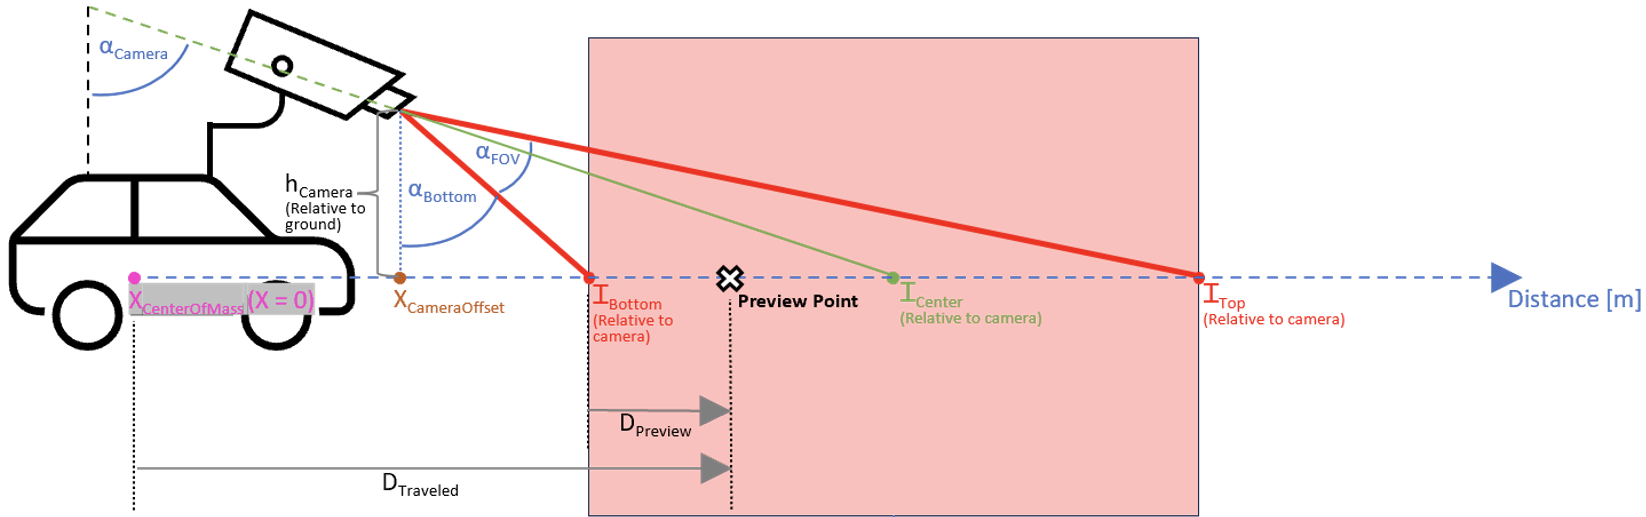
\includegraphics[width=1\linewidth]{Pictures/Bildschirmfoto 2024-02-05 um 01.49.52.png}
    \caption{Skizze der nötigen Parameter für die Berechnung der Vorschauweite}
    \label{fig:skizze_parameter_vorschauweite}
\end{figure}

Die Bestimmung der Vorschauweite ist jedoch mit der Einschränkung verbunden, dass sie nicht beliebig klein werden kann, da der untere Bildrand die minimale Vorschauweite vorgibt. Somit kann bei sehr langsamen Fahrten die Vorschauweite minimal auf die Distanz des unteren Bildrandes gesetzt werden. 


\subsection{Bestimmen von Parametern}
\autor{Felix Anslinger}

Das genaue Bestimmen von gewissen Parametern ist notwendig, damit der Regler bestmöglich funktionieren kann. Für die, in den vorherigen Kapiteln beschriebene, Implementierung des Stanley-Reglers, wird das genaue Bestimmen der Totzeit \(T_{dead}\), sowie der Montageposition der Kamera durch \(h_{Camera}\) und \(X_{CameraOffset}\), vorausgesetzt. 
Für das Bestimmen von solchen Parametern, empfiehlt es sich abzuwarten, bis alle finalen Hardwareänderungen an dem Fahrzeug vollbracht wurden. Andernfalls können sich die Parameter durch weitere Hardwareänderungen im Nachhinein ändern und müssten demnach erneut bestimmt werden.
